
%%%%%%%%%%%%%%%%%%%%%%%%%%%%%%%%%%%%%%%%%%%%%%%%%%%%%%%%%%%%%%%%%%%%%%%%%%%%%%%
%
%  EGSnrc manual: system considerations
%  Copyright (C) 2015 National Research Council Canada
%
%  This file is part of EGSnrc.
%
%  EGSnrc is free software: you can redistribute it and/or modify it under
%  the terms of the GNU Affero General Public License as published by the
%  Free Software Foundation, either version 3 of the License, or (at your
%  option) any later version.
%
%  EGSnrc is distributed in the hope that it will be useful, but WITHOUT ANY
%  WARRANTY; without even the implied warranty of MERCHANTABILITY or FITNESS
%  FOR A PARTICULAR PURPOSE.  See the GNU Affero General Public License for
%  more details.
%
%  You should have received a copy of the GNU Affero General Public License
%  along with EGSnrc. If not, see <http://www.gnu.org/licenses/>.
%
%%%%%%%%%%%%%%%%%%%%%%%%%%%%%%%%%%%%%%%%%%%%%%%%%%%%%%%%%%%%%%%%%%%%%%%%%%%%%%%
%
%  Author:          Iwan Kawrakow, 2003
%
%  Contributors:    Blake Walters
%                   Frederic Tessier
%                   Ernesto Mainegra-Hing
%
%%%%%%%%%%%%%%%%%%%%%%%%%%%%%%%%%%%%%%%%%%%%%%%%%%%%%%%%%%%%%%%%%%%%%%%%%%%%%%%


%This is not a stand alone file   it is an input to pirs701.tex
% This started from nrc_egs4_primer_for_beam (SID 1.13 last edited 22 May 1998)
% 				SID 1.1 was as found Sept 16 1996
\typeout{Start of  using_egsnrc_system}

% Replace line with fixed date with the one below when commiting
% Beware: Using the macro below conflicts between CVS and latex!!!
% \lfoot[{\sffamily {\leftmark}}]{{\small Last edited $Date: 2013/03/27 14:07:42 $
\lfoot[{\sffamily {\leftmark}}]{{\small Last edited 2011/03/09 20:45:06
}}

\section{EGSnrc System Considerations}
\label{sys_consid}

This section is almost completely superceded by Report PIRS-877 which
describes the EGSnrcMP environment or system for using the EGSnrc
system\cite{Ka03}.  This section is left here for old time's sake! A few of
the specific commands have been updated to avoid total confusion.
\subsection{Introduction}

\index{.egs4inp} \index{egsnp} \index{\$EGS\_HOME}
The EGSnrc Code System works in a manner which is very similar to the EGS4
system so that those using the EGS4 system already should find this very
familiar.  The major changes are to make
the user codes subdirectories of \verb+$EGS_HOME+ instead of  \verb+$HOME/egs4+ and to
define the files related to specific runs as \verb+.egsinp+ instead of
\verb+.egs4inp+ etc.  These changes have been made to make it possible to
run both systems in parallel for a while when making the transition, and to
clearly identify which system various files refer to.  This can be done by
merely changing the definition  of the environment variable {\tt
HEN\_HOUSE} to point at either the EGSnrc or the EGS4 area,
and sourcing {\tt Cshrc\_additions\_for\_egsnrc} instead of {\tt
Cshrc\_additions\_for\_egs4} in your {\tt .cshrc} file. If you are already
an \verb+EGS_pert+ then the rest of this section will be of little
interest.  If you are new to EGS and the above makes no sense at all, then
this is the section for you!


\subsection{Overview}

The EGSnrc system, which was originally developed for Unix based systems by
Alex Bielajew, is very flexible and powerful.  This comes at the expense of
being somewhat complicated at first sight.  However, the scripts which come
with the system make it quite easy to use and flexible once you are familiar
with the over-all design.
\index{Bielajew, Alex}

The EGSnrc system consists of two major directory area.
One area, the \verb+HEN_HOUSE+, holds all the standard EGSnrc files
and does not get changed. The structure of the \verb+HEN_HOUSE+ is
shown in fig~\ref{fig_hen_house_2}.  The \verb+HEN_HOUSE+ can be maintained
anywhere on the system that all local EGSnrc users can read. One useful
approach in a multi-user environment is to have a user called {\tt egsnrc} and
make the \verb+HEN_HOUSE+ the {\tt \$HOME}  directory of that user. If you
are the only local EGSnrc user, you can make the \verb+HEN_HOUSE+ a
subdirectory of your {\tt \$HOME} area.  In either case, when you initiate
the {\tt INSTALL\_EGS} procedure, you should do so on the directory
where you want the \verb+HEN_HOUSE+ to reside (see section~\ref{install} on
page ~\pageref{install} for more on installation).
\index{installation}
\index{INSTALL\_EGS}
\index{HEN\_HOUSE}
\vspace*{-0.4cm}
\begin{figure}[h]
\index{HEN\_HOUSE}
%\htmlimage{scale=1.6}   %this makes it readable
\begin{center}
\leavevmode
\mbox{}\hspace{-1cm}
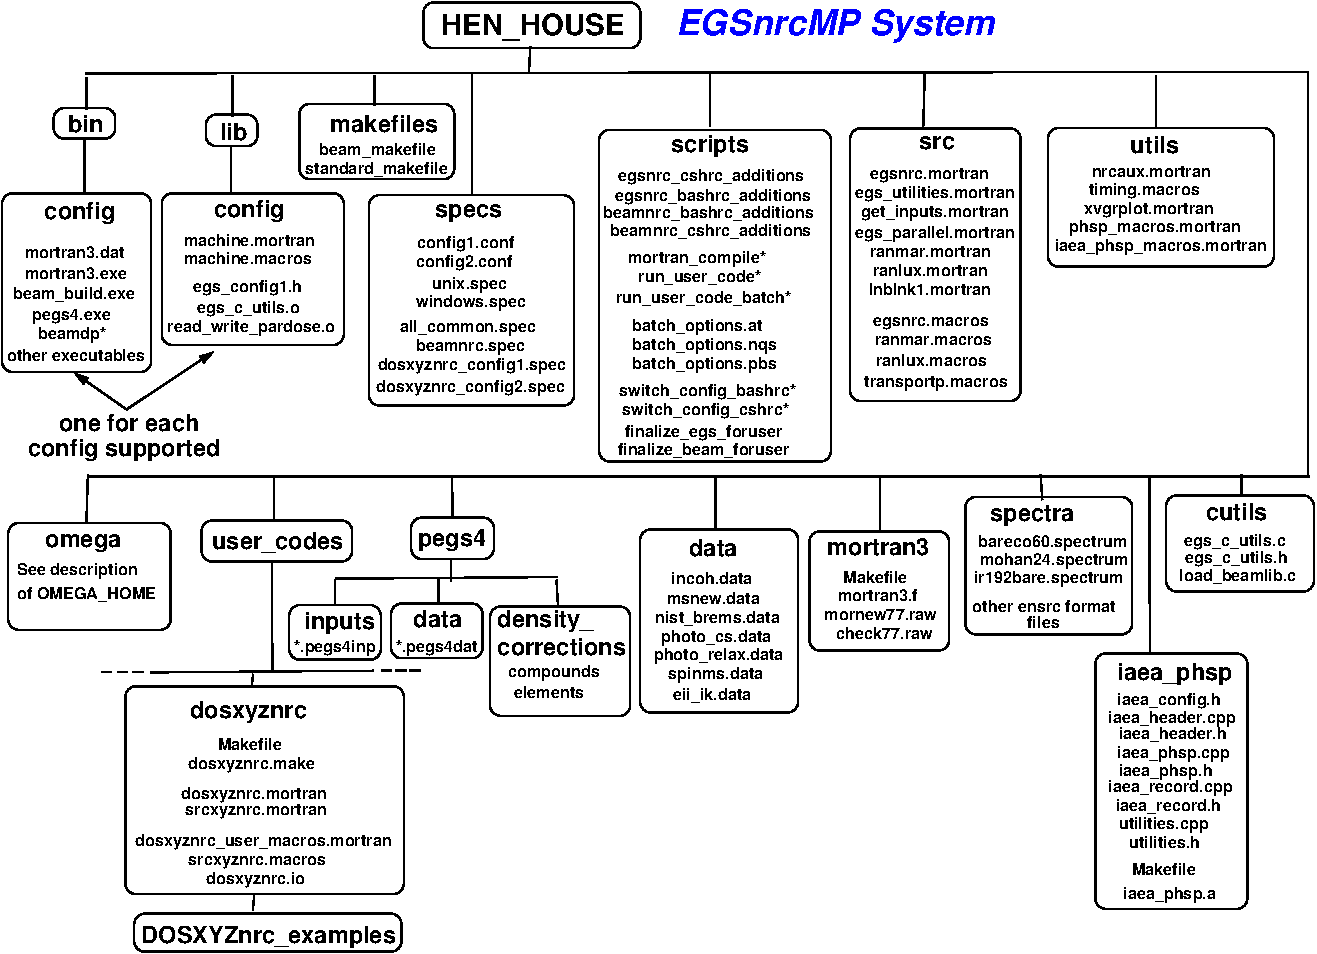
\includegraphics[width=15cm]{figures/egsnrc_system}
    \caption[Components of the {\tt HEN\_HOUSE} area for the EGSnrc
system.]
{The components of the {\tt HEN\_HOUSE} area for the EGSnrc
system. There are also subdirectories related to documentation and
NRC user codes which are not shown here and the main {\tt HEN\_HOUSE} box
actually has multiple subdirectories which are not shown. See PIRS-877 for
details\cite{Ka03}.}
\label{fig_hen_house_2}
\end{center}
\end{figure}

\clearpage

%\index{\$EGS\_HOME}
%\index{EGS\_HOME}
The second major  directory area of the EGSnrc system is
on the individual user's area and holds all the user's user codes and run associated
files.
It is mandatory that you set up a subdirectory which is referred to as
\verb+$EGS_HOME+ (e.g.,  frequently \verb+$HOME/egsnrc+) and for
each \verb+user_code.mortran+ which you use or write, there must be a sub-directory with
the same name as the user code, \ie~ \verb+$EGS_HOME/user_code+.
A typical user's area is shown in figure~\ref{fig_nrc_users_area}.
\begin{figure}[htb]
%\htmlimage{scale=1.6}   %this makes it readable
%\index{\$EGS\_HOME}
%\index{EGS\_HOME}
\index{EGSnrc!users area}
\index{user's area}
\begin{center}
\index{NRC EGSnrc user's area}
\index{user's area}
\leavevmode
\mbox{}\hspace{-1cm}
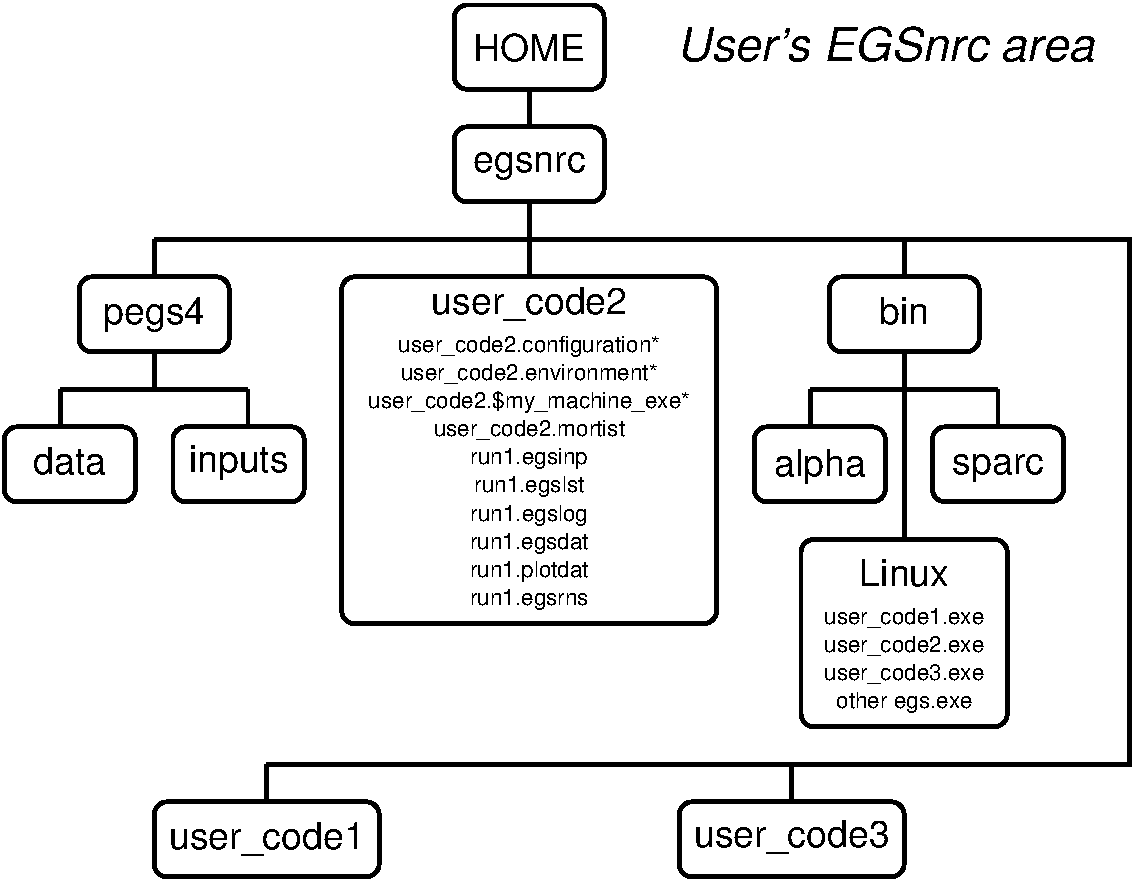
\includegraphics[width=14cm]{figures/users_egsnrc_area}
 \caption{Components of a typical EGS user's area where, for this
 example, {\tt \$EGS\_HOME} is {\tt \$HOME/egsnrc}. On a given system
 there can be an arbitrary number of different user's areas.
 \label{fig_nrc_users_area}
 }
\end{center}
\end{figure}

\subsubsection{A complication for multi-architecture systems}
\index{multi-architecture system}
% At NRC we run with a variety of different machines, all of which access
% a single disk system.  The EGSnrc system is set up to handle this
% transparently but this adds an additional level of complexity to the
% underlying system.  The system keeps track of which machine you are on
% at all times and uses the appropriate execute modules \etc.  This aspect
% of things is handled by the variable \verb+my_machine+ which essentially
% identifies the type of cpu currently being used and is determined by the
% script \verb+$HEN_HOUSE/get_machine+. The system is set up to store the
% executable files (the {\tt .exe}  files) on separate disk areas for each
% type of machine. To execute the code on different machine you must first
% compile it on each type of machine you want to use.  As new machines come
% along, the script \verb+$HEN_HOUSE/get_machine+ may become out of date and
% users may have to update it to return appropriate information for their
% system and more importantly, adjust the run and compile scripts to use the
% appropriate switches for their machine.
% \index{my\_machine}
% \index{get\_machine}
The install scripts are clever enough to establish various machine or
compiler dependencies and create the files {\tt
\$HEN\_HOUSE/lib/{my\_config}/machine.macros} and\\
 {\tt \$HEN\_HOUSE/lib/{my\_config}/machine.mortran} where {\tt
{my\_config}} is the name of your particular configuration (eg, g77,
gfortran, Mac).

\subsubsection{System aliases and environment variables}
\index{aliases} \index{environment variables}
\index{Cshrc\_additions\_for\_egsnrc}
\index{.login} \index{.cshrc}
\index{shell to use}
The EGSnrc system is based on using {\tt csh} C-shell scripts or {\tt sh},
bash shell scripts and to
facilitate this one should run from the C-shell ({\tt csh} or {\tt tcsh})
or the bash shell {\tt sh}.
To define the
aliases and other variables needed by the system, there are files called
{\tt egsnrc\_cshrc\_additions} and {\tt egsnrc\_bashrc\_additions} available on
{\tt \$HEN\_HOUSE/scripts}.
However, one first needs to set the environment variable {\tt HEN\_HOUSE}
to point at the location of the {\tt HEN\_HOUSE}. This is most conveniently
done with a declaration in your {\tt .login} file or {\tt .cshrc} file or
{\tt .bashrc} file depending on which shell is your default.
\begin{verbatim}
      setenv HEN_HOUSE location_of_HEN_HOUSE (e.g. $HOME/HEN_HOUSE)
\end{verbatim}
or for {\tt .bashrc}
\begin{verbatim}
      HEN_HOUSE=/absolute_location_of_your_HEN_HOUSE/ (e.g. $HOME/HEN_HOUSE)
\end{verbatim}
Then it is {\bfseries essential} that in your {\tt .cshrc} or {\tt .bashrc}
file you source the
{\tt  egsnrc\_cshrc\_additions} or {\tt egsnrc\_bashrc\_additions} file, i.e. add the statement:
\begin{verbatim}
     source $HEN_HOUSE/scripts/egsnrc_cshrc_additions}
\end{verbatim}
or, for those using {\tt bash}:
\begin{verbatim}
     source $HEN_HOUSE/scripts/egsnrc_bashrc_additions}
or
     source /absolute_location_of_your_HEN_HOUSE/scripts/egsnrc_bashrc_additions}
\end{verbatim}

These additions file set up many aliases and other variables for you. These
are most easily seen by executing the commands {\tt alias}, {\tt set} and
{\tt setenv} although this will show you all of the systems definitions as
well.  We will explain the use of many of these definitions in the
remainder of this section but the most important of the aliases are:
\index{egsnrc\_cshrc\_additions}
\index{egsnrc\_bashrc\_additions}

\index{mf} \index{mor} \index{f} \index{f} \index{ex} \index{mfb}
\index{PEGS4} \index{examin} \index{Mortran3!mor mf m}
\begin{description}
\item[mor]	MORTRAN a stand alone code
\item[m]	MORTRAN a specified users code
\item[mf]	MORTRAN and Fortran compile and link a specified users code
\item[f]	Fortran compile and link a specified users code
\item[ex]	execute an egs user code
\item[exb]	execute an egs user code in batch mode
%\item[pegs4]	run pegs4 (see section~\ref{pegs4_sc})
%\item[examin]   examin a particular data set from pegs4
%above not inlcuded now.
\end{description}
The use of these is described below in detail but note that the command
{\tt make} is now the easiest way to mortran and fortran user codes as
described in PIRS-877\cite{Ka03}.

% This script no longer here
%% The script {\tt
%% show\_settings} (on {\tt \$HEN\_HOUSE}) gives a more or less complete list
%% of all aliases, variables and environment variable associated
%% with EGSnrc once {\tt Cshrc\_additons\_for\_egsnrc} has been sourced. For
%% more detail see section~\ref{settings} (page~\pageref{settings}).
%% \index{show\_settings} \index{settings}



\newpage
\subsection{PEGS4}
\index{PEGS4}
\label{pegs4_sc}

As described elsewhere in this report, PEGS4 is the program which
prepares much of the material dependent cross section data sets required
by EGSnrc to do the simulations (see section~\ref{pegs4} on
page~\pageref{pegs4}).  As discussed there, use of the {\tt egs\_gui}
greatly facilitates the use of the {\tt PEGS4} program.

\index{.pegs4dat}
\index{.pegs4inp}
\index{densities for PEGS4}
The user must have the directories {\tt \$EGS\_HOME/pegs4},
{\tt \$EGS\_HOME/pegs4/inputs} and {\tt \$EGS\_HOME/pegs4/data}.
A user's PEGS4 input file is on {\tt \$EGS\_HOME/pegs4/inputs}
and has the name \verb+my_data.pegs4inp+.  The PEGS4 program outputs the
data file for EGSnrc to
\verb+$EGS_HOME/pegs4/data/my_data.pegs4dat+.
The listing file from the PEGS4
run is found on \verb+$EGS_HOME/pegs4+ and is called \verb+my_data.pegslst+.
To invoke PEGS4 one enters:
\begin{verbatim}
pegs4.exe -i inputfile [-o ofile] [-a] [-d density] [-x crosssection] [-e HEN_HOUSE]

inputfile.pegs4inp   the input file
output defaults to $HEN_HOUSE/pegs4/data/inputfile.pegs4dat
                or, if ofile is given, to $HEN_HOUSE/pegs4/data/ofile.pegs4dat
[-a]            => append results to output file
[-d density]    => use density.density   for density effect
[-x crosssection] => use $HEN_HOUSE/pegs4/crosssection instead of
                                $HEN_HOUSE/pegs4/pgs4pepr.dat
[-e HEN_HOUSE]  => use this absolute location as the HEN_HOUSE
\end{verbatim}
where \verb+my_data.pegsinp+ is the input file described in detail in
section~\ref{pegs4_input} (page~\pageref{pegs4_input}) and
\verb+density.density+
is a file containing the density effect information needed for this
particular calculation IF it is needed by \verb+my_data.pegsinp+.
The PEGS4 script checks the following directories, in order, for
the file \verb+density.density+.
\begin{verbatim}
$EGS_HOME/pegs4/inputs
$EGS_HOME/pegs4/density_corrections/elements
$EGS_HOME/pegs4/density_corrections/compounds
$EGS_HOME/pegs4/density_corrections
$HEN_HOUSE/pegs4/density_corrections/elements
$HEN_HOUSE/pegs4/density_corrections/compounds
\end{verbatim}

\subsubsection{Where pegs4 data is kept}
\index{PEGS4!where data is kept}
\index{.pegs4dat}
\label{wpdk}

Note that PEGS4 can only create one material output file per run and
if the simulation you want to run requires data for more than one material,
these must be joined into one \verb+file.pegs4dat+ file, either by
concatenation, by using an editor or by the {\tt -a} option in the command
line.

The EGSnrc run scripts look for the data file requested (see
section~\ref{Execution}), first on\\
\verb+$EGS_HOME/pegs4/data+ and if not
found there, then it looks on \verb+$HEN_HOUSE/pegs4/data+.
\vfill

\subsubsection{examin}
\index{EXAMIN}
The command:\\
\verb+examin -p file+
\\(note there is no ``e'' at the end of \verb+examin+) will allow you
to plot and/or list much of the photon and electron cross section data
in the file \verb+$EGS_HOME/pegs4/data/file.pegs4dat+ or if that is not
present, then in the file \verb+$HEN_HOUSE/pegs4/data/file.pegs4dat+. Note that
\verb+examin+ no longer displays the photon cross section data from the
PEGS4 data file but displays the data actually used by EGSnrc. The default
dataset used by \verb+examin+ is xcom. If you are using something else in your
user code, you must change the following line in the code:

\verb+REPLACE {$XDATA-DEFAULT} WITH {'xcom'}+

The output is found on \verb+$EGS_HOME/examin+. If requested, during execution
\verb+examin+ pops open \verb+xmgrace+ (a 2-D graphing package), otherwise
you have to use the listing files created. See section~\ref{examin}
(page ~\pageref{examin}).
\index{xmgrace}

\subsection{Compilation (MORTRAN and Fortran)}
\index{compiling}
\label{Compilation}

\index{Mortran3}

The EGSnrc system is written in the Mortran3 language which is
a pre-processor for Fortran.  Mortran3 is itself written in
Fortran.  The Mortran3 processor is part of the EGSnrc
distribution and is discussed in detail in section~\ref{UGM3},
page~\pageref{UGM3} of this report.  In order to create an executable file
from the mortran source files, there are two steps needed. The first step,
converts the mortran source code into standard Fortran77. We call this {\tt
MORTRAN} compiling.  The next step turns the Fortran source into an
executable, using the standard Fortran compile and link process.

Using the EGSnrcMP system (see PIRS-877\cite{Ka03}), the most direct way to
do these steps is using the {\tt make} command.  The following are the old
way to do it but they still work.

To ``compile'' the user code {\tt user\_code.mortran}, one issues the command:\\
\index{mf}\index{m}
\verb+mf user_code a [opt0|opt1|opt2|opt3|opt4]+\\
or\\
\verb+m user_code+\\

\index{Mortran3}
\index{Fortran}
The \verb+mf+ command will MORTRAN, Fortran and link the
entire user-code called \verb+user_code+, including the EGSnrc
system.  The Fortran and the execute modules are machine specific (SUN vs
SGI vs Linux etc) but this is handled in a transparent manner by the scripts.

The \verb+m+ command will MORTRAN the entire user-code
called \verb+user_code+, including the EGSnrc system. The output is
a Fortran file \verb+user_code_{my_machine}.f+ which is specific for the
machine being used since the script picks up a set of macros which
handles any differences between the machines.

The \verb+f+ command will Fortran and link the entire
Fortran version of the user-code called
\verb+user_code_{my_machine}.f+, which includes the EGSnrc system.
The scripts automatically detect the value for \verb+my_machine+ and use
the appropriate value.

\verb+user_code.mortran+ or \verb+user_code_{my_machine}.f+
must be present on area \\
\verb+$EGS_HOME/user_code+.

\index{compiling!options}
The letter {\tt a} after the user code name is a residual option which no
longer exists, but which has been left for compatibility with
a wide range of other scripts at NRC.  This option was associated with a
technique to avoid recompiling unchanged Fortran subroutines from one pass
to the next, but this was removed since compilers have become so fast that
it was not very useful and occasionally led to problems and always left
many extra files around. Note that  the
standard \verb+make+ facility does not work because the date on the Fortran
file is
always more recent than that on the object module since MORTRAN creates
a new version of the Fortran each time.


The option \verb+[opt0|opt1|opt2|opt3|opt4|debug]+ allows selection of
the optimisation level to be used.  For production codes, be sure to use
at least \verb+opt2+ since these can save up to 50\% over
\verb+opt0+, but they usually take much longer to compile and link.

\subsubsection{The  user\_code.configuration file (obsolete)}
\index{configuration file}
\index{.configuration file}
This approach has been completely revised and replaced by the {\tt
user\_code.make} file with {\tt SOURCES = } formats. See
PIRS-877\cite{Ka03}.  The same general capabilities have been maintained
in the new format.

During the MORTRAN stage, the scripts still create a file, called
\verb+.mortjob.mortran+ on \\
\verb+$EGS_HOME/user_code+. This file
contains all the source code for this
particular user\_code (macros, user\_code, and
any other routines the user wants, etc).
The files which are concatenated together to
form \verb+.mortjob.mortran+ are defined by the user.
% in the file\\
% \verb+$EGS_HOME/user_code/user_code.configuration+.  If this file is
% not present, the script uses the generic
% \verb+$HEN_HOUSE/standard.configuration+.  Figure~\ref{std_config} presents
% a listing of this file.
% \begin{latexonly}
% \input{standard.configuration}
% \end{latexonly}
% \begin{htmlonly}
% \clearpage
% \input{standard.configuration_html}
% \clearpage
% \end{htmlonly}



The {\tt .configuration} file (or new equivalent {\tt .make} file) allows for
very flexible options when compiling a given user
code.  For example, it is possible to change which random number generator
is being used throughout the system by merely changing which pair of files
are included in the configuration file, either {\tt ranlux.macros} and {\tt
ranlux.mortran} or {\tt ranmar.macros} and {\tt ranmar.mortran} (see
section~\ref{rngs}, page~\pageref{rngs}). However if
anything other than the default seeds and luxury levels are desired, there
may be some minor changes needed n {\tt user\_code.mortran}
unless one is very careful (\eg\ DOSRZnrc is designed to use either rng).
\index{RANMAR} \index{RANLUX}

\subsubsection{Order is Important}

The following still applies. When the file {\tt .mortjob.mortran} is
created, the order in which the various files are placed in the file is
important.  This is primarily because in Mortran3 the last definition of
any macro is the one that is in force.  Thus it is important that the {\tt
egsnrc.macros} file be read in early since this defines all of the default
values of the macros.  As long as it appears before the user code, then any
macro redefinitions done in the user code take precedence.

% the following no longer works so I removed the section
% \subsubsection{Batch compilations}
% \index{compiling!in batch}
% \index{batch!compiling}
% \index{batch}
% To compile in batch, just add a \verb+b+ to the above commands,
% \ie~\verb+mfb+ \etc. This will submit the compilation to whatever batch
% system you are using (see section~\ref{batch_que}).

\subsubsection{{\tt machine.mortran} files}
\index{machine.mortran}
Different compilers often have slightly different ways of handling certain
things.  The most common differences are regarding how files are opened
(i.e., the format of the {\tt OPEN} statement), and what is more difficult,
how they handle time.  EGSnrc itself has very few of these constructs
within it, but the user codes cannot avoid them.  To overcome these
differences, there are a series of macros defined in {\tt machine.mortran}
files which are found on {\tt
\$HEN\_HOUSE/lib/\$my\_machine/machine.mortran}.  It is even more complex
for Linux machines where the {\tt machine.mortran} files differ depending
on what version of the compiler you are using.  The default settings are
for a fairly recent {\tt g77} compiler but if you are using a slightly
older one you may need to edit the {\tt egs\_compile} script to select a
different default for the variable {\tt Linux\_compiler}.
\index{Linux\_compiler}

The {\tt  machine.mortran} files define a macro {\tt \$MACHINE} which the
user codes pick up. It is useful to define this properly in the {\tt
machine.mortran} which is picked up in your local environment.
\index{machine.mortran}
\index{\$MACHINE}

The above requirements are handled by a {\tt machine.mortran} which is
created for your system by the EGSnrcMP system as described in PIRS-877.


% no longer relevant so removed
% \subsubsection{{\tt get\_machine}, what if it fails?}
% \index{{get\_machine}}
% The script {\tt get\_machine} is designed to tell the EGSnrc scripts what
% type of machine is being used.  If the system you are using is not
% recognised by the scripts, it will try to compile using pretty vanilla
% flavoured compiler and loader flags.  The script will print out what flags
% it is using.  If you wish to change these to match the requirements of your
% machine, edit the {\tt egs\_compile} script. You may want to hard wire the
% selection of {\tt my\_flags} and {\tt my\_libs} to match your own
% machine/compiler.  If it is a common, new machine or compiler, please
% let us know what
% settings were needed and we will try to fit them into the next release.  We
% also hope to clean up these scripts and allow a more direct method to
% modify/tailor the system.
%



\subsection{Execution}
\index{execution}
\label{Execution}
\index{.egsinp}

The following works mostly still,, but there are new ways described in
PIRS-877\cite{Ka03} for the EGSnrcMP system.


Once a user code has been compiled, it is executed by issuing:

\hspace*{1cm}\verb+ex[b] user_code input data [queue|debug]+\vspace*{5mm}\\
\verb+$EGS_HOME/user_code/input.egsinp+ and\\
\verb+$EGS_HOME/user_code/user_code.{my_machine}_exe+ must exist.  The
PEGS4 data is in \verb+data.pegs4dat+ \index{.pegs4dat}which is located either on
the users area or the system area, as discussed in section~\ref{wpdk}.

\index{execution in batch}
If \verb+queue+ is not specified when the batch option ``{\tt b}'' is being
used, then the default queue on your system is used.
\index{interactive execution}

\index{debug}
In interactive mode, the 4-th input can be \verb+debug+ if a debug run
is wanted.  There must be an execute module created with the debug
switch set during compilation for this to work.

Execution of EGSnrc jobs is handled by the script {\tt egs\_run}
which is on the {\tt HEN\_HOUSE}.

At the completion of the run, all output and batch output files are
found on\\
\verb+$EGS_HOME/user_code/+ unless the user has specified something
different in the environment file (see below).

\index{execution!subdirectory during}
\index{subdirectory  during execution}
During execution, the {\tt egs\_run} script creates a separate subdirectory area
and only modifies the files there. This is usually a subdirectory of
\verb+$EGS_HOME/user_code/+ but on a Linux system is on {\tt /tmp}
(this is to
make the subdirectory local to the machine running the job since on the NRC
system, having the disk on another machine would seriously slow down the
job). All
the files are moved back to \verb+$EGS_HOME/user_code/+ after
completion of the run.  This can be confusing unless you are aware of this
behaviour.

\subsubsection{user\_code.environment file (obsolete)}
\index{.environment file}
\index{environment file}

This functionality is reworked and described in PIRS-877\cite{Ka03}.  In
particular the {\tt user\_code.io} file is relevant although the general
ideas below are still applicable.

% The execution scripts source
% \verb+$EGS_HOME/user_code/user_code.environment+ immediately prior to
% executing the \verb+user_code+ and then again immediately after.  An
% example  is given in
% \verb+$HEN_HOUSE/example_usercode.environment+ which is shown in
% figure~\ref{ex_environment}.  In general, this file defines the links to
% specific files from Fortran units, \etc.
%
Almost all Fortran compilers associate a file called {\tt fort.n} with any I/O
unit {\tt n} which is not attached explicitly within the code to some
file name. Thus if {\tt HATCH} read data from unit 12 without any open
statement, then it looks for {\tt fort.12}.  The system must associate
this file name to the real file name.
There are a series of similar links established
for files which have common names for all user codes.

% \begin{latexonly}
% \input{example_usercode.environment}
% \end{latexonly}
% \begin{htmlonly}
% \clearpage
% \input{example_usercode.environment_html}
% \clearpage
% \end{htmlonly}




The following files are associated with a normal type of run with an NRC
user code (although the environment files can add whatever files the user
may want and the files below are not mandatory).  For
this example, the input file name is \verb+input.egsinp+.
\begin{description}
\item [input.egsinp:] defined by the user.
\item [input.egslst:]  the output listing file from the run. Erased
at start of next run if not renamed.
\item [input.egslog:] The log file which echos the inputs and
prompts when running in batch. Note, this has most of the {\bf error}
messages too, so get in the habit of reading this file.
\item [input.egsdat:] A file containing all the information needed to
allow a calculation to be restarted again.
\item [input.egsrns:] Some codes allow a record of random number seeds
at the start of each history to be kept (just most recent). These are
kept in this file if requested.
\item [input.egsplot (etc):] Plotting files for various routines, the
most up to date are for \verb+xmgrace+.
\index{xmgrace}
\item [input.egsgeom:] file with output description of geometry for
\verb+EGS_windows+.
\item [input.egsgph:] file with output phase space of each history for
\verb+EGS_windows+.
\end{description}

% The one known exception to the rule above about {\tt fort.n} files names is the
% HP unix system.  Here the default Fortran unit name is {\tt ftn05} for {\tt
% fort.5} etc. The approach here is to use statements like {\tt setenv ftn11
% fort.11} in the {\tt .environment} file prior to the link statement. This
% is done within {\tt egs\_run} for  many units which are regularly used.

\subsubsection{Batch Queues (obsolete)}
\label{batch_que}
See PIRS-877 for how this is handled now.


\subsection{Parallel Processing}
\label{pprocess}
\index{pprocess}
\index{parallel processing}
\index{NQS}

The following is replaced by a more sophisticated approach in the EGSnrcMP
system and the standard NRC user codes. See PIRS-877\cite{Ka03}.

Monte Carlo calculations with EGSnrc are easily run in parallel and the
results combined at the end of the runs because every history is completely
independent, as long as the random number sequences are independent. One of
the reasons for selecting the random number generators distributed with
EGSnrc is that there is a simple procedure for ensuring independent
sequences (see section~\ref{rngs} on page~\pageref{rngs}).

The NRC user codes\cite{Ro00} have a parallel processing option built in.
The system used requires the NQS batch submission system to be installed on
all machines to be run in parallel. The option is implemented via a script,
called {\tt pprocess} which makes an arbitrary number of input files from
the original file, ensuring different random number sequences for each and
then submitting the job to an arbitrary number of machines.  At the end of
the runs, the main user code is run once more with instructions to combine
the results of the previous runs.  Although crude, it is highly effective.
We routinely run using more than 30 of our 38 CPUs running in parallel.
The script {\tt combine\_egsnrc} has been written to automatically edit the
required input file and execute the needed final run for the analysis of
parallel runs with the NRC user codes.
There is more discussion in reference~\cite{Ro00}.
\index{combine\_egsnrc}

Note that there is a useful script called {\tt
clean\_after\_parallel} which is found on\newline {\tt \$HEN\_HOUSE/scripts}.
Parallel runs create a huge number of files and this script helps clean
them up, but only once they have been analysed.
\index{clean\_after\_parallel}


\subsection{Distribution / Installation of EGSnrc}
\label{install}
\index{distribution}
\index{installation}
\index{Cshrc\_additions\_for\_egsnrc}
\index{INSTALL\_EGS}


\index{.cshrc}
\index{HEN\_HOUSE}
This installation script requires that the environment variables
\verb+HEN_HOUSE+ not be defined when the script is called and not be
defined in the user's {\tt .cshrc} or {\tt .bashrc} file. The installation will create
the entire \verb+$HEN_HOUSE+ structure shown in
fig~\ref{fig_hen_house_2} (page~\pageref{fig_hen_house_2})
and compile a variety of codes for the machine
the user is doing the installation from (\viz\ Mortran3,
PEGS4, DOSRZnrc).  It also partially sets up the user's area
\verb+$EGS_HOME+.

Once the \verb+INSTALL_EGS+ script has been successfully executed, one
must ensure that the environment variables {\tt HEN\_HOUSE} and {\tt
EGS\_HOME} are defined to
point at wherever you have placed the EGSnrc system and your EGSnrc user
area.

Most importantly, the installation leaves behind a file called
\verb+egsnrc_cshrc_additions+ or \verb+egsnrc_bashrc_additions+
which MUST be sourced from the user's
{\tt .cshrc} script or {\tt .bashrc} script depending on which default
shell is used. Once the installation is complete,
add the following to your {\tt .cshrc} file:\\
\verb+source /explicit_path_to_your_HEN_HOUSE/egsnrc_cshrc_additions+. \\
or the following to your {\tt .bashrc} file:\\
\verb+source /explicit_path_to_your_HEN_HOUSE/egsnrc_bashrc_additions+. \\
\index{egsnrc\_bashrc\_additions}
\index{egsnrc\_cshrc\_additions}

The user should try to run the {\tt tutor} codes to ensure the system is working.

% For examples of the files created by {\tt INSTALL\_EGS}, see\\
% {\tt \$HEN\_HOUSE/test\_distribution\_outputs}.
% \index{example lst\_install files}
%
% One can also run the script {\tt test\_distribution} (see
% section~\ref{test_distribution}, page~\pageref{test_distribution}) which
% exercises the system extensively.
% \index{test\_distribution}.


% \subsection{On-Line Manuals}
% \index{on-line manuals}
% The manuals for the EGSnrc system are on-line from the same site as the
% distribution.
% \subsection{Changes and bugs corrected since initial release}
% \label{fixed_bugs}
% \index{bugs}
% \index{corrected bugs}
%
% %%%%%%%%%%%%%%%%%%%%%%%%%%%%%%%%%%%%%%%%%%%%%%%%%%%%%%%%%%%%%%%%%%%%%%%%%%%
% \noindent The following changes were made to EGSnrc in a minor release in Oct, 2001
% %%%%%%%%%%%%%%%%%%%%%%%%%%%%%%%%%%%%%%%%%%%%%%%%%%%%%%%%%%%%%%%%%%%%%%%%%%%
% \begin{itemize}
% \item A call to AUSGAB immediately prior to annihilation of a positron at
% rest was added with IARG=28.
%
% \item The auxiliary input routine for EGSnrc parameters was changed to use
% macros to define the defaults.
%
% \item A change was made to allow {\tt skindepth\_for\_bca} to be less than
% 1.
% \item James Tickner pointed out that K-alpha1 and K-alpha2 transition
% probabilities had been inverted.  This was fixed.
%
% \end{itemize}
%
% \noindent The following changes were made to EGSnrc in the May, 2001 release.
% \begin{itemize}
% \item WT = 0.0 now causes new particles to be discarded immediately via the
% \\
% {\tt USER-PHOTON-DISCARD} and {\tt USER-ELECTRON-DISCARD} exits which
% generate {\tt IARG = 3} exits.  This saves time and avoids other problems
% (see section~\ref{termination}, page~\pageref{termination}).
% \item {\tt \$COMIN-RELAX} is now defined in {\tt egsnrc.macros} instead of
% in {\tt subroutine relax}.
% \end{itemize}
%
% %%%%%%%%%%%%%%%%%%%%%%%%%%%%%%%%%%%%%%%%%%%%%%%%%%%%%%%%%%%%%%%%%%%%%%%%%%%
% \noindent The following bugs in EGSnrc were fixed in the May, 2002 release.
% %%%%%%%%%%%%%%%%%%%%%%%%%%%%%%%%%%%%%%%%%%%%%%%%%%%%%%%%%%%%%%%%%%%%%%%%%%%
%
% \begin{itemize}
% \item If using the SLAC geometry macros, the COMIN's did not contain the
% needed declarations of the variables.
% \item Daniel Frei from Bern pointed out an error which affected a charged
% particle going directly backwards along the Z axis.
% \item Format of the region number output by {\tt subroutine WATCH} was
% changed so that it would work for region numbers greater than 9,999. The
% original format caused {\tt EGS\_Windows} to misbehave.
% \item Alex Bielajew pointed out that egs\_batch does not work when using the
% standard at batch command due to extra white space.
% \item Permissions on data sets are changed to allow world read access.
% \item Omar Chibani pointed out that the density scaling didn't work
% properly. This has been fixed and the manual also made clearer.
% \item History by history statistical analysis was implemented in all user
% codes.
% \end{itemize}
%
% %%%%%%%%%%%%%%%%%%%%%%%%%%%%%%%%%%%%%%%%%%%%%%%%%%%%%%%%%%%%%%%%%%%%%%%%%%%
% \noindent The following bugs in EGSnrc were fixed in the Nov., 2003 release.
% %%%%%%%%%%%%%%%%%%%%%%%%%%%%%%%%%%%%%%%%%%%%%%%%%%%%%%%%%%%%%%%%%%%%%%%%%%%
%
%
% \begin{itemize}
% \item Many improvements to the GUI's and the entire new EGSnrcMP
% environment (see Report PIRS-877\cite{Ka03} for an extensive discussion).
%
% \item Fixed the ranlux RNG so that restarting a specific history is now
% possible (useful for debugging purposes).
%
% \item Fixed a bug pointed out by Rebecca Nutbrown re normalization of
% results when a phase-space source was recycled.
%
% \item Fixed a bug in FLURZnrc.mortran regarding electron fluence in bins
% below ECUT.
%
% \item Fixed a serious normalization bug in DOSRZnrc for the case where
% parallel runs were done using a phase-space source. The bug was pointed
% out by Roberto Capote who also pointed out a similar sort of bug which
% applied to all the RZ codes when using a phase space source and recycling
% the source.
%
% \item Bug in the {\tt preview3d} code for use with EGS\_Windows for
% cylindrical geometries was fixed.
%
% \item A bug, which was pointed out by Wamied Abdel-Rahman and Frank Verhaegen
% regarding positron annihilation when using the NIST cross sections for
% bremsstrahlung	production, was fixed.
%
% \item A bug related to discards for being below ECUT and PCUT in a vacuum
% was fixed.
% \end{itemize}
%
%
%
% \subsection{Known bugs/restrictions}
% \index{Known bugs}
% \index{restrictions}
%
% Straggling in the continuous energy loss is not modelled.
%
